\documentclass{beamer}

\usepackage{cmap}
\usepackage[english,russian]{babel} % add eng,rus(base) package
\usepackage[T1,T2A]{fontenc}        % add eng,rus encoding support
\usepackage[utf8]{inputenc}         % add UTF8 support

% Use it for English document
%\usepackage[utf8]{inputenc} % add UTF8 support
%\usepackage{fontspec}       % to use any font known to the operating system
%\setmainfont{PT Serif}      % set defolt font

\usepackage{amsmath, amsfonts, amssymb, amsthm, mathtools} % add math support

\linespread{1}               % length between str
\setlength{\parindent}{16pt} % red str
\setlength{\parskip}{6pt}   % length between paragraphs

\usepackage[backend=biber, style=authoryear-icomp]{biblatex}
\addbibresource{$HOME/latex-templates/biblio.bib}            % path to bibliography base

\usetheme{Madrid}
\setbeamertemplate{frametitle}[default][center]

\renewcommand{\thefootnote}{\arabic{footnote}}
 % here is document's settings for russian


\title{Вторая чеченская война}
\author{Немков Н.М.}
\institute[МГТУ]{МГТУ им. Н.Э. Баумана}
\date{06.05.2024}

\begin{document}

\begin{frame}
\maketitle
\end{frame}


%=============================== 1
\begin{frame}{}


	Первая чеченская война, завершившаяся Хасавюртовскими соглашениями, не принесла заметных улучшений на территорию Чечни.



	В 1999 году боевики Басаева и Хаттаба попытались провести военную операцию в Дагестане, что и послужило основным поводом для начала новой войны. В то же самое время были проведены теракты в Буйнакске, Москве и Волгодонске.
%	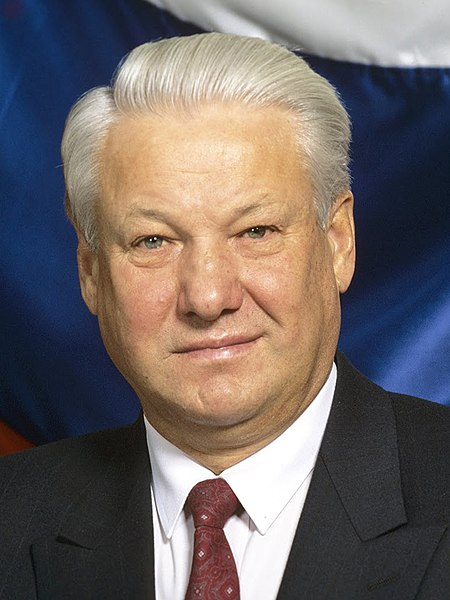
\includegraphics[width=1\textwidth]{images/elcin-1}

\end{frame}

%================================ 2
\section{}
\begin{frame}{}
	\textbf{1999 год}

	 7 августа -- Вторжение боевиков в Дагестан

	4–16 августа -- Теракты в Буйнакске, Москве, Волгодонске

	18 августа -- Блокирование границ с Чечней

	23 сентября -- Указ Б. Ельцина «О мерах по повышению эффективности контртеррористических операций на территории Северо-Кавказского региона Российской Федерации»

	30 сентября -- Федеральные войска вошли на территорию Чечни

	26 декабря -- Начало штурма Грозного

	\textbf{2000 год}

	6 февраля -- Завершение операции по освобождению Грозного

	\textbf{2009 год}

	15 апреля -- Отмена режима контртеррористической операции в Чечне

\end{frame}


%================================ 3
%================================ 4
\section{}
\begin{frame}{}

Планируя вторжение на территорию Дагестана, боевики надеялись на поддержку местного населения, но оно оказало им отчаянное сопротивление.

За август 1999 года чеченские бандформирования были выбиты с территории Дагестана

23 сентября федеральная авиация начала бомбардировку Грозного, а уже 30 сентября войска вошли на территорию Чечни.

\end{frame}


%================================ 6
\section{}
\begin{frame}{}

26 декабря 1999 года началась операция по ликвидации бандформирований в Грозном. Бои продолжались весь январь 2000 года, и только 6 февраля было объявлено о полном освобождении города.

\end{frame}


%================================ 7
\section{Итоги}
\begin{frame}{Итоги}

	Главным итогом Второй чеченской войны можно считать достигнутое относительное спокойствие в Чеченской Республике.

	Был положен конец криминальному разгулу, терроризировавшему население в течение десяти лет.

	Была ликвидирована наркоторговля и работорговля.

	на Кавказе не удалось реализовать планы исламистов по созданию мировых центров террористических организаций.

\end{frame}


\section{Благоданость}
\begin{frame}
	\centering
	\huge
	Спасибо за внимание!
\end{frame}


\end{document}
